% Options for packages loaded elsewhere
% Options for packages loaded elsewhere
\PassOptionsToPackage{unicode}{hyperref}
\PassOptionsToPackage{hyphens}{url}
%
\documentclass[
  english,
  russian,
  12pt,
  a4paper,
  DIV=11,
  numbers=noendperiod]{scrartcl}
\usepackage{xcolor}
\usepackage{amsmath,amssymb}
\setcounter{secnumdepth}{5}
\usepackage{iftex}
\ifPDFTeX
  \usepackage[T1]{fontenc}
  \usepackage[utf8]{inputenc}
  \usepackage{textcomp} % provide euro and other symbols
\else % if luatex or xetex
  \usepackage{unicode-math} % this also loads fontspec
  \defaultfontfeatures{Scale=MatchLowercase}
  \defaultfontfeatures[\rmfamily]{Ligatures=TeX,Scale=1}
\fi
\usepackage{lmodern}
\ifPDFTeX\else
  % xetex/luatex font selection
\fi
% Use upquote if available, for straight quotes in verbatim environments
\IfFileExists{upquote.sty}{\usepackage{upquote}}{}
\IfFileExists{microtype.sty}{% use microtype if available
  \usepackage[]{microtype}
  \UseMicrotypeSet[protrusion]{basicmath} % disable protrusion for tt fonts
}{}
\usepackage{setspace}
\makeatletter
\@ifundefined{KOMAClassName}{% if non-KOMA class
  \IfFileExists{parskip.sty}{%
    \usepackage{parskip}
  }{% else
    \setlength{\parindent}{0pt}
    \setlength{\parskip}{6pt plus 2pt minus 1pt}}
}{% if KOMA class
  \KOMAoptions{parskip=half}}
\makeatother
% Make \paragraph and \subparagraph free-standing
\makeatletter
\ifx\paragraph\undefined\else
  \let\oldparagraph\paragraph
  \renewcommand{\paragraph}{
    \@ifstar
      \xxxParagraphStar
      \xxxParagraphNoStar
  }
  \newcommand{\xxxParagraphStar}[1]{\oldparagraph*{#1}\mbox{}}
  \newcommand{\xxxParagraphNoStar}[1]{\oldparagraph{#1}\mbox{}}
\fi
\ifx\subparagraph\undefined\else
  \let\oldsubparagraph\subparagraph
  \renewcommand{\subparagraph}{
    \@ifstar
      \xxxSubParagraphStar
      \xxxSubParagraphNoStar
  }
  \newcommand{\xxxSubParagraphStar}[1]{\oldsubparagraph*{#1}\mbox{}}
  \newcommand{\xxxSubParagraphNoStar}[1]{\oldsubparagraph{#1}\mbox{}}
\fi
\makeatother

\usepackage{color}
\usepackage{fancyvrb}
\newcommand{\VerbBar}{|}
\newcommand{\VERB}{\Verb[commandchars=\\\{\}]}
\DefineVerbatimEnvironment{Highlighting}{Verbatim}{commandchars=\\\{\}}
% Add ',fontsize=\small' for more characters per line
\usepackage{framed}
\definecolor{shadecolor}{RGB}{241,243,245}
\newenvironment{Shaded}{\begin{snugshade}}{\end{snugshade}}
\newcommand{\AlertTok}[1]{\textcolor[rgb]{0.68,0.00,0.00}{#1}}
\newcommand{\AnnotationTok}[1]{\textcolor[rgb]{0.37,0.37,0.37}{#1}}
\newcommand{\AttributeTok}[1]{\textcolor[rgb]{0.40,0.45,0.13}{#1}}
\newcommand{\BaseNTok}[1]{\textcolor[rgb]{0.68,0.00,0.00}{#1}}
\newcommand{\BuiltInTok}[1]{\textcolor[rgb]{0.00,0.23,0.31}{#1}}
\newcommand{\CharTok}[1]{\textcolor[rgb]{0.13,0.47,0.30}{#1}}
\newcommand{\CommentTok}[1]{\textcolor[rgb]{0.37,0.37,0.37}{#1}}
\newcommand{\CommentVarTok}[1]{\textcolor[rgb]{0.37,0.37,0.37}{\textit{#1}}}
\newcommand{\ConstantTok}[1]{\textcolor[rgb]{0.56,0.35,0.01}{#1}}
\newcommand{\ControlFlowTok}[1]{\textcolor[rgb]{0.00,0.23,0.31}{\textbf{#1}}}
\newcommand{\DataTypeTok}[1]{\textcolor[rgb]{0.68,0.00,0.00}{#1}}
\newcommand{\DecValTok}[1]{\textcolor[rgb]{0.68,0.00,0.00}{#1}}
\newcommand{\DocumentationTok}[1]{\textcolor[rgb]{0.37,0.37,0.37}{\textit{#1}}}
\newcommand{\ErrorTok}[1]{\textcolor[rgb]{0.68,0.00,0.00}{#1}}
\newcommand{\ExtensionTok}[1]{\textcolor[rgb]{0.00,0.23,0.31}{#1}}
\newcommand{\FloatTok}[1]{\textcolor[rgb]{0.68,0.00,0.00}{#1}}
\newcommand{\FunctionTok}[1]{\textcolor[rgb]{0.28,0.35,0.67}{#1}}
\newcommand{\ImportTok}[1]{\textcolor[rgb]{0.00,0.46,0.62}{#1}}
\newcommand{\InformationTok}[1]{\textcolor[rgb]{0.37,0.37,0.37}{#1}}
\newcommand{\KeywordTok}[1]{\textcolor[rgb]{0.00,0.23,0.31}{\textbf{#1}}}
\newcommand{\NormalTok}[1]{\textcolor[rgb]{0.00,0.23,0.31}{#1}}
\newcommand{\OperatorTok}[1]{\textcolor[rgb]{0.37,0.37,0.37}{#1}}
\newcommand{\OtherTok}[1]{\textcolor[rgb]{0.00,0.23,0.31}{#1}}
\newcommand{\PreprocessorTok}[1]{\textcolor[rgb]{0.68,0.00,0.00}{#1}}
\newcommand{\RegionMarkerTok}[1]{\textcolor[rgb]{0.00,0.23,0.31}{#1}}
\newcommand{\SpecialCharTok}[1]{\textcolor[rgb]{0.37,0.37,0.37}{#1}}
\newcommand{\SpecialStringTok}[1]{\textcolor[rgb]{0.13,0.47,0.30}{#1}}
\newcommand{\StringTok}[1]{\textcolor[rgb]{0.13,0.47,0.30}{#1}}
\newcommand{\VariableTok}[1]{\textcolor[rgb]{0.07,0.07,0.07}{#1}}
\newcommand{\VerbatimStringTok}[1]{\textcolor[rgb]{0.13,0.47,0.30}{#1}}
\newcommand{\WarningTok}[1]{\textcolor[rgb]{0.37,0.37,0.37}{\textit{#1}}}

\usepackage{longtable,booktabs,array}
\usepackage{calc} % for calculating minipage widths
% Correct order of tables after \paragraph or \subparagraph
\usepackage{etoolbox}
\makeatletter
\patchcmd\longtable{\par}{\if@noskipsec\mbox{}\fi\par}{}{}
\makeatother
% Allow footnotes in longtable head/foot
\IfFileExists{footnotehyper.sty}{\usepackage{footnotehyper}}{\usepackage{footnote}}
\makesavenoteenv{longtable}
\usepackage{graphicx}
\makeatletter
\newsavebox\pandoc@box
\newcommand*\pandocbounded[1]{% scales image to fit in text height/width
  \sbox\pandoc@box{#1}%
  \Gscale@div\@tempa{\textheight}{\dimexpr\ht\pandoc@box+\dp\pandoc@box\relax}%
  \Gscale@div\@tempb{\linewidth}{\wd\pandoc@box}%
  \ifdim\@tempb\p@<\@tempa\p@\let\@tempa\@tempb\fi% select the smaller of both
  \ifdim\@tempa\p@<\p@\scalebox{\@tempa}{\usebox\pandoc@box}%
  \else\usebox{\pandoc@box}%
  \fi%
}
% Set default figure placement to htbp
\def\fps@figure{htbp}
\makeatother



\ifLuaTeX
\usepackage[bidi=basic,provide=*]{babel}
\else
\usepackage[bidi=default,provide=*]{babel}
\fi
% get rid of language-specific shorthands (see #6817):
\let\LanguageShortHands\languageshorthands
\def\languageshorthands#1{}


\setlength{\emergencystretch}{3em} % prevent overfull lines

\providecommand{\tightlist}{%
  \setlength{\itemsep}{0pt}\setlength{\parskip}{0pt}}



 


\KOMAoption{captions}{tableheading}
\makeatletter
\@ifpackageloaded{caption}{}{\usepackage{caption}}
\AtBeginDocument{%
\ifdefined\contentsname
  \renewcommand*\contentsname{Содержание}
\else
  \newcommand\contentsname{Содержание}
\fi
\ifdefined\listfigurename
  \renewcommand*\listfigurename{Список иллюстраций}
\else
  \newcommand\listfigurename{Список иллюстраций}
\fi
\ifdefined\listtablename
  \renewcommand*\listtablename{Список таблиц}
\else
  \newcommand\listtablename{Список таблиц}
\fi
\ifdefined\figurename
  \renewcommand*\figurename{Рисунок}
\else
  \newcommand\figurename{Рисунок}
\fi
\ifdefined\tablename
  \renewcommand*\tablename{Таблица}
\else
  \newcommand\tablename{Таблица}
\fi
}
\@ifpackageloaded{float}{}{\usepackage{float}}
\floatstyle{ruled}
\@ifundefined{c@chapter}{\newfloat{codelisting}{h}{lop}}{\newfloat{codelisting}{h}{lop}[chapter]}
\floatname{codelisting}{Список}
\newcommand*\listoflistings{\listof{codelisting}{Листинги}}
\makeatother
\makeatletter
\makeatother
\makeatletter
\@ifpackageloaded{caption}{}{\usepackage{caption}}
\@ifpackageloaded{subcaption}{}{\usepackage{subcaption}}
\makeatother
\usepackage{bookmark}
\IfFileExists{xurl.sty}{\usepackage{xurl}}{} % add URL line breaks if available
\urlstyle{same}
\hypersetup{
  pdftitle={Отчёт по лабораторной работе №2},
  pdfauthor={Улитина Мария Максимовна},
  pdflang={ru-RU},
  hidelinks,
  pdfcreator={LaTeX via pandoc}}


\title{Отчёт по лабораторной работе №2}
\usepackage{etoolbox}
\makeatletter
\providecommand{\subtitle}[1]{% add subtitle to \maketitle
  \apptocmd{\@title}{\par {\large #1 \par}}{}{}
}
\makeatother
\subtitle{Имитационное моделирование}
\author{Улитина Мария Максимовна}
\date{}
\begin{document}
\maketitle

\renewcommand*\contentsname{Содержание}
{
\setcounter{tocdepth}{2}
\tableofcontents
}
\listoffigures
\listoftables

\setstretch{1.5}
\section{Цель
работы}\label{ux446ux435ux43bux44c-ux440ux430ux431ux43eux442ux44b}

Цель данной лабораторной работы --- подготовить рабочее пространство для
выполнения программ и приобрести необходимые навыки создания и
преобразования программ на Julia.

\section{Задание}\label{ux437ux430ux434ux430ux43dux438ux435}

\begin{itemize}
\tightlist
\item
  Создать рабочий каталог для всего курса.
\item
  Создать рабочее пространство для программ в рамках лабораторной
  работы.
\item
  Выполнить все задания по тексту лабораторной работы.
\item
  Установить необходимые пакеты.
\item
  Выполнить предложенный код.
\item
  Преобразовать код в литературный стиль.
\item
  Сгенерировать из литературного кода:

  \begin{itemize}
  \tightlist
  \item
    чистый код;
  \item
    jupyter notebook;
  \item
    документацию в формате Quarto.
  \item
    Выполнить код из jupyter notebook.
  \end{itemize}
\item
  Интегрировать документацию в формате Quarto в отчёт.
\item
  Добавить в код в литературном стиле вычисление для набора параметров.
\item
  Сгенерировать из литературного кода с параметрами:

  \begin{itemize}
  \tightlist
  \item
    чистый код;
  \item
    jupyter notebook;
  \item
    документацию в формате Quarto.
  \item
    Выполнить код из jupyter notebook с параметрами.
  \end{itemize}
\item
  Интегрировать документацию с параметрами в формате Quarto в отчёт.
\end{itemize}

\section{Выполнение лабораторной
работы}\label{ux432ux44bux43fux43eux43bux43dux435ux43dux438ux435-ux43bux430ux431ux43eux440ux430ux442ux43eux440ux43dux43eux439-ux440ux430ux431ux43eux442ux44b}

\subsection{Создание рабочего каталога
курса}\label{ux441ux43eux437ux434ux430ux43dux438ux435-ux440ux430ux431ux43eux447ux435ux433ux43e-ux43aux430ux442ux430ux43bux43eux433ux430-ux43aux443ux440ux441ux430}

Создаём репозиторий на основе шаблона (рис.~\ref{fig-001}).

\begin{figure}

\centering{

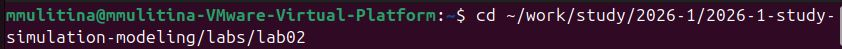
\includegraphics[width=0.7\linewidth,height=\textheight,keepaspectratio]{image/1.jpg}

}

\caption{\label{fig-001}Создание рабочего каталога}

\end{figure}%

Инициализируем проект (рис.~\ref{fig-002}).

\begin{figure}

\centering{

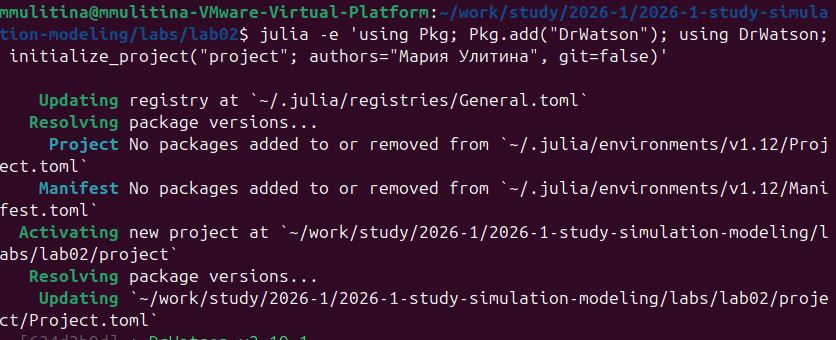
\includegraphics[width=0.7\linewidth,height=\textheight,keepaspectratio]{image/2.jpg}

}

\caption{\label{fig-002}Инициализация проекта}

\end{figure}%

Загрузим необходимые пакеты (рис.~\ref{fig-003}).

\begin{figure}

\centering{

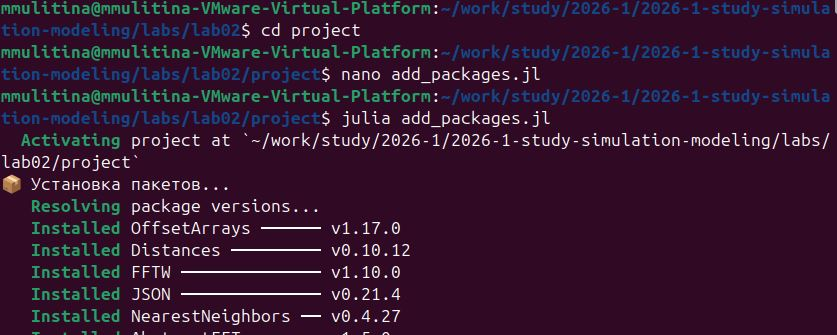
\includegraphics[width=0.7\linewidth,height=\textheight,keepaspectratio]{image/3.jpg}

}

\caption{\label{fig-003}Установка пакетов}

\end{figure}%

Создадим необходимые скрипты (рис.~\ref{fig-004}).

\begin{figure}

\centering{

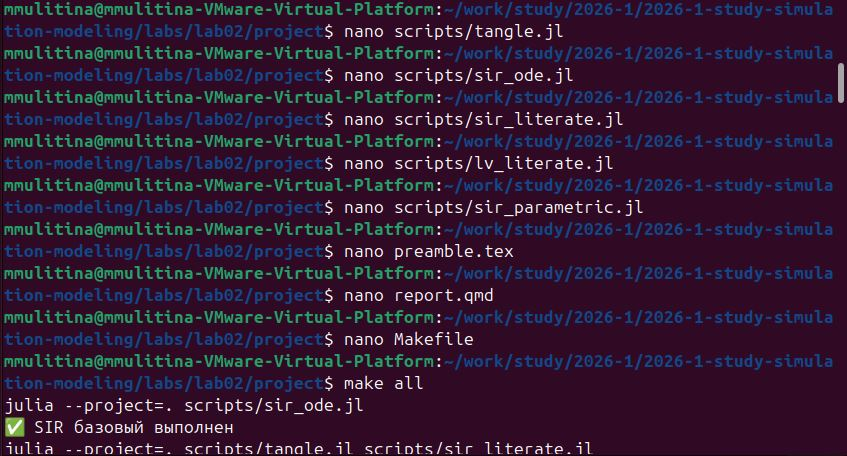
\includegraphics[width=0.7\linewidth,height=\textheight,keepaspectratio]{image/4.jpg}

}

\caption{\label{fig-004}Создание скриптов}

\end{figure}%

Отправим изменения в git (рис.~\ref{fig-005}).

\begin{figure}

\centering{

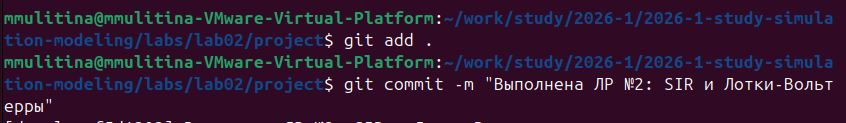
\includegraphics[width=0.7\linewidth,height=\textheight,keepaspectratio]{image/5.jpg}

}

\caption{\label{fig-005}git}

\end{figure}%

\section{Модель
Лотки-Вольтерры}\label{ux43cux43eux434ux435ux43bux44c-ux43bux43eux442ux43aux438-ux432ux43eux43bux44cux442ux435ux440ux440ux44b}

Уравнения: \[
\begin{cases}
\frac{dx}{dt} = \alpha x - \beta x y \\
\frac{dy}{dt} = \delta x y - \gamma y
\end{cases}
\]

\begin{Shaded}
\begin{Highlighting}[]
\ImportTok{using} \BuiltInTok{DrWatson}
\PreprocessorTok{@quickactivate} \StringTok{"project"}
\ImportTok{using} \BuiltInTok{DifferentialEquations}\NormalTok{, }\BuiltInTok{DataFrames}\NormalTok{, }\BuiltInTok{Plots}\NormalTok{, }\BuiltInTok{LaTeXStrings}

\NormalTok{script\_name }\OperatorTok{=} \FunctionTok{splitext}\NormalTok{(}\FunctionTok{basename}\NormalTok{(}\ConstantTok{PROGRAM\_FILE}\NormalTok{))[}\FloatTok{1}\NormalTok{]}
\FunctionTok{mkpath}\NormalTok{(}\FunctionTok{plotsdir}\NormalTok{(script\_name))}

\KeywordTok{function} \FunctionTok{lotka\_volterra!}\NormalTok{(du, u, p, t)}
\NormalTok{    x, y }\OperatorTok{=}\NormalTok{ u}
\NormalTok{    α, β, δ, γ }\OperatorTok{=}\NormalTok{ p}
\NormalTok{    du[}\FloatTok{1}\NormalTok{] }\OperatorTok{=}\NormalTok{ α}\OperatorTok{*}\NormalTok{x }\OperatorTok{{-}}\NormalTok{ β}\OperatorTok{*}\NormalTok{x}\OperatorTok{*}\NormalTok{y}
\NormalTok{    du[}\FloatTok{2}\NormalTok{] }\OperatorTok{=}\NormalTok{ δ}\OperatorTok{*}\NormalTok{x}\OperatorTok{*}\NormalTok{y }\OperatorTok{{-}}\NormalTok{ γ}\OperatorTok{*}\NormalTok{y}
    \ConstantTok{nothing}
\KeywordTok{end}

\NormalTok{prob\_lv }\OperatorTok{=} \FunctionTok{ODEProblem}\NormalTok{(lotka\_volterra!, [}\FloatTok{40.0}\NormalTok{, }\FloatTok{9.0}\NormalTok{], (}\FloatTok{0.0}\NormalTok{, }\FloatTok{200.0}\NormalTok{), [}\FloatTok{0.1}\NormalTok{, }\FloatTok{0.02}\NormalTok{, }\FloatTok{0.01}\NormalTok{, }\FloatTok{0.3}\NormalTok{])}
\NormalTok{sol\_lv }\OperatorTok{=} \FunctionTok{solve}\NormalTok{(prob\_lv, }\FunctionTok{Tsit5}\NormalTok{(), dt}\OperatorTok{=}\FloatTok{0.1}\NormalTok{)}

\NormalTok{df\_lv }\OperatorTok{=} \FunctionTok{DataFrame}\NormalTok{(t}\OperatorTok{=}\NormalTok{sol\_lv.t, prey}\OperatorTok{=}\NormalTok{[u[}\FloatTok{1}\NormalTok{] for u }\KeywordTok{in}\NormalTok{ sol\_lv.u], pred}\OperatorTok{=}\NormalTok{[u[}\FloatTok{2}\NormalTok{] for u }\KeywordTok{in}\NormalTok{ sol\_lv.u])}

\NormalTok{plt1 }\OperatorTok{=} \FunctionTok{plot}\NormalTok{(df\_lv.t, [df\_lv.prey df\_lv.pred], label}\OperatorTok{=}\NormalTok{[L}\StringTok{"x"}\NormalTok{ L}\StringTok{"y"}\NormalTok{], title}\OperatorTok{=}\StringTok{"Динамика"}\NormalTok{, lw}\OperatorTok{=}\FloatTok{2}\NormalTok{)}
\FunctionTok{savefig}\NormalTok{(plt1, }\FunctionTok{plotsdir}\NormalTok{(script\_name, }\StringTok{"lv\_dyn.png"}\NormalTok{))}

\NormalTok{plt2 }\OperatorTok{=} \FunctionTok{plot}\NormalTok{(df\_lv.prey, df\_lv.pred, title}\OperatorTok{=}\StringTok{"Фазовый портрет"}\NormalTok{, xlabel}\OperatorTok{=}\StringTok{"Жертвы"}\NormalTok{, ylabel}\OperatorTok{=}\StringTok{"Хищники"}\NormalTok{, lw}\OperatorTok{=}\FloatTok{2}\NormalTok{)}
\FunctionTok{savefig}\NormalTok{(plt2, }\FunctionTok{plotsdir}\NormalTok{(script\_name, }\StringTok{"lv\_phase.png"}\NormalTok{))}
\end{Highlighting}
\end{Shaded}

\begin{verbatim}
┌ Warning: DrWatson could not find find a project file by recursively checking given `dir` and its parents. Returning `nothing` instead.
│ (given dir: /home/mmulitina)
└ @ DrWatson ~/.julia/packages/DrWatson/2QF5p/src/project_setup.jl:84
\end{verbatim}

\begin{verbatim}
"/home/mmulitina/work/study/2026-1/2026-1-study-simulation-modeling/labs/lab02/report/plots/lv_phase.png"
\end{verbatim}

\section{Модель SIR
(Susceptible-Infectious-Recovered)}\label{ux43cux43eux434ux435ux43bux44c-sir-susceptible-infectious-recovered}

\textbf{Цель:} Исследование динамики эпидемии. Уравнения: \[
\begin{cases}
\frac{dS}{dt} = -\beta c \frac{I}{N} S \\
\frac{dI}{dt} = \beta c \frac{I}{N} S - \gamma I \\
\frac{dR}{dt} = \gamma I
\end{cases}
\]

\begin{Shaded}
\begin{Highlighting}[]
\ImportTok{using} \BuiltInTok{DrWatson}
\PreprocessorTok{@quickactivate} \StringTok{"project"}
\ImportTok{using} \BuiltInTok{DifferentialEquations}\NormalTok{, }\BuiltInTok{DataFrames}\NormalTok{, }\BuiltInTok{Plots}\NormalTok{, }\BuiltInTok{LaTeXStrings}

\NormalTok{script\_name }\OperatorTok{=} \FunctionTok{splitext}\NormalTok{(}\FunctionTok{basename}\NormalTok{(}\ConstantTok{PROGRAM\_FILE}\NormalTok{))[}\FloatTok{1}\NormalTok{]}
\FunctionTok{mkpath}\NormalTok{(}\FunctionTok{plotsdir}\NormalTok{(script\_name))}

\KeywordTok{function} \FunctionTok{sir\_ode!}\NormalTok{(du, u, p, t)}
\NormalTok{    S, I, R }\OperatorTok{=}\NormalTok{ u}
\NormalTok{    β, c, γ }\OperatorTok{=}\NormalTok{ p}
\NormalTok{    N }\OperatorTok{=}\NormalTok{ S }\OperatorTok{+}\NormalTok{ I }\OperatorTok{+}\NormalTok{ R}
\NormalTok{    du[}\FloatTok{1}\NormalTok{] }\OperatorTok{=} \OperatorTok{{-}}\NormalTok{β }\OperatorTok{*}\NormalTok{ c }\OperatorTok{*}\NormalTok{ I }\OperatorTok{/}\NormalTok{ N }\OperatorTok{*}\NormalTok{ S}
\NormalTok{    du[}\FloatTok{2}\NormalTok{] }\OperatorTok{=}\NormalTok{ β }\OperatorTok{*}\NormalTok{ c }\OperatorTok{*}\NormalTok{ I }\OperatorTok{/}\NormalTok{ N }\OperatorTok{*}\NormalTok{ S }\OperatorTok{{-}}\NormalTok{ γ }\OperatorTok{*}\NormalTok{ I}
\NormalTok{    du[}\FloatTok{3}\NormalTok{] }\OperatorTok{=}\NormalTok{ γ }\OperatorTok{*}\NormalTok{ I}
    \ConstantTok{nothing}
\KeywordTok{end}

\NormalTok{prob }\OperatorTok{=} \FunctionTok{ODEProblem}\NormalTok{(sir\_ode!, [}\FloatTok{990.0}\NormalTok{, }\FloatTok{10.0}\NormalTok{, }\FloatTok{0.0}\NormalTok{], (}\FloatTok{0.0}\NormalTok{, }\FloatTok{40.0}\NormalTok{), [}\FloatTok{0.05}\NormalTok{, }\FloatTok{10.0}\NormalTok{, }\FloatTok{0.25}\NormalTok{])}
\NormalTok{sol }\OperatorTok{=} \FunctionTok{solve}\NormalTok{(prob, dt }\OperatorTok{=} \FloatTok{0.1}\NormalTok{)}

\NormalTok{df }\OperatorTok{=} \FunctionTok{DataFrame}\NormalTok{(t}\OperatorTok{=}\NormalTok{sol.t, S}\OperatorTok{=}\NormalTok{[u[}\FloatTok{1}\NormalTok{] for u }\KeywordTok{in}\NormalTok{ sol.u], I}\OperatorTok{=}\NormalTok{[u[}\FloatTok{2}\NormalTok{] for u }\KeywordTok{in}\NormalTok{ sol.u], R}\OperatorTok{=}\NormalTok{[u[}\FloatTok{3}\NormalTok{] for u }\KeywordTok{in}\NormalTok{ sol.u])}
\NormalTok{plt }\OperatorTok{=} \FunctionTok{plot}\NormalTok{(df.t, [df.S df.I df.R], label}\OperatorTok{=}\NormalTok{[L}\StringTok{"S"}\NormalTok{ L}\StringTok{"I"}\NormalTok{ L}\StringTok{"R"}\NormalTok{], title}\OperatorTok{=}\StringTok{"Модель SIR"}\NormalTok{, lw}\OperatorTok{=}\FloatTok{2}\NormalTok{)}
\FunctionTok{savefig}\NormalTok{(plt, }\FunctionTok{plotsdir}\NormalTok{(script\_name, }\StringTok{"sir\_lit.png"}\NormalTok{))}
\end{Highlighting}
\end{Shaded}

\begin{verbatim}
┌ Warning: DrWatson could not find find a project file by recursively checking given `dir` and its parents. Returning `nothing` instead.
│ (given dir: /home/mmulitina)
└ @ DrWatson ~/.julia/packages/DrWatson/2QF5p/src/project_setup.jl:84
\end{verbatim}

\begin{verbatim}
"/home/mmulitina/work/study/2026-1/2026-1-study-simulation-modeling/labs/lab02/report/plots/sir_lit.png"
\end{verbatim}

\section{Параметрическое исследование
SIR}\label{ux43fux430ux440ux430ux43cux435ux442ux440ux438ux447ux435ux441ux43aux43eux435-ux438ux441ux441ux43bux435ux434ux43eux432ux430ux43dux438ux435-sir}

\begin{Shaded}
\begin{Highlighting}[]
\ImportTok{using} \BuiltInTok{DrWatson}
\PreprocessorTok{@quickactivate} \StringTok{"project"}
\ImportTok{using} \BuiltInTok{DifferentialEquations}\NormalTok{, }\BuiltInTok{DataFrames}\NormalTok{, }\BuiltInTok{Plots}

\NormalTok{script\_name }\OperatorTok{=} \FunctionTok{splitext}\NormalTok{(}\FunctionTok{basename}\NormalTok{(}\ConstantTok{PROGRAM\_FILE}\NormalTok{))[}\FloatTok{1}\NormalTok{]}
\FunctionTok{mkpath}\NormalTok{(}\FunctionTok{plotsdir}\NormalTok{(script\_name))}

\KeywordTok{function} \FunctionTok{sir\_ode!}\NormalTok{(du, u, p, t)}
\NormalTok{    S, I, R }\OperatorTok{=}\NormalTok{ u}
\NormalTok{    β, c, γ }\OperatorTok{=}\NormalTok{ p}
\NormalTok{    N }\OperatorTok{=}\NormalTok{ S }\OperatorTok{+}\NormalTok{ I }\OperatorTok{+}\NormalTok{ R}
\NormalTok{    du[}\FloatTok{1}\NormalTok{] }\OperatorTok{=} \OperatorTok{{-}}\NormalTok{β }\OperatorTok{*}\NormalTok{ c }\OperatorTok{*}\NormalTok{ I }\OperatorTok{/}\NormalTok{ N }\OperatorTok{*}\NormalTok{ S}
\NormalTok{    du[}\FloatTok{2}\NormalTok{] }\OperatorTok{=}\NormalTok{ β }\OperatorTok{*}\NormalTok{ c }\OperatorTok{*}\NormalTok{ I }\OperatorTok{/}\NormalTok{ N }\OperatorTok{*}\NormalTok{ S }\OperatorTok{{-}}\NormalTok{ γ }\OperatorTok{*}\NormalTok{ I}
\NormalTok{    du[}\FloatTok{3}\NormalTok{] }\OperatorTok{=}\NormalTok{ γ }\OperatorTok{*}\NormalTok{ I}
    \ConstantTok{nothing}
\KeywordTok{end}

\NormalTok{beta\_values }\OperatorTok{=}\NormalTok{ [}\FloatTok{0.02}\NormalTok{, }\FloatTok{0.05}\NormalTok{, }\FloatTok{0.08}\NormalTok{, }\FloatTok{0.12}\NormalTok{]}
\NormalTok{plt }\OperatorTok{=} \FunctionTok{plot}\NormalTok{(title}\OperatorTok{=}\StringTok{"Влияние β на I(t)"}\NormalTok{, xlabel}\OperatorTok{=}\StringTok{"Время"}\NormalTok{, ylabel}\OperatorTok{=}\StringTok{"I(t)"}\NormalTok{)}

\ControlFlowTok{for}\NormalTok{ β }\KeywordTok{in}\NormalTok{ beta\_values}
\NormalTok{    prob }\OperatorTok{=} \FunctionTok{ODEProblem}\NormalTok{(sir\_ode!, [}\FloatTok{990.0}\NormalTok{, }\FloatTok{10.0}\NormalTok{, }\FloatTok{0.0}\NormalTok{], (}\FloatTok{0.0}\NormalTok{, }\FloatTok{40.0}\NormalTok{), [β, }\FloatTok{10.0}\NormalTok{, }\FloatTok{0.25}\NormalTok{])}
\NormalTok{    sol }\OperatorTok{=} \FunctionTok{solve}\NormalTok{(prob, }\FunctionTok{Tsit5}\NormalTok{())}
    \FunctionTok{plot!}\NormalTok{(plt, sol.t, [u[}\FloatTok{2}\NormalTok{] for u }\KeywordTok{in}\NormalTok{ sol.u], label}\OperatorTok{=}\StringTok{"β = }\SpecialCharTok{$}\StringTok{β", }\NormalTok{lw}\StringTok{=2)}
\ControlFlowTok{end}

\FunctionTok{savefig}\NormalTok{(plt, }\FunctionTok{plotsdir}\NormalTok{(script\_name, }\StringTok{"beta\_sens.png"}\NormalTok{))}
\end{Highlighting}
\end{Shaded}

\begin{verbatim}
┌ Warning: DrWatson could not find find a project file by recursively checking given `dir` and its parents. Returning `nothing` instead.
│ (given dir: /home/mmulitina)
└ @ DrWatson ~/.julia/packages/DrWatson/2QF5p/src/project_setup.jl:84
\end{verbatim}

\begin{verbatim}
"/home/mmulitina/work/study/2026-1/2026-1-study-simulation-modeling/labs/lab02/report/plots/beta_sens.png"
\end{verbatim}

\section{Выводы}\label{ux432ux44bux432ux43eux434ux44b}

В ходе выполнения лабораторной работы была реализована Модель SIR -
модель эпидемиологии, описывающая распространение инфекционного
заболевания в закрытой популяции.

\section{Источники}\label{ux438ux441ux442ux43eux447ux43dux438ux43aux438}

{[}1{]} W. O. Kermack and A. G. McKendrick, ``A Contribution to the
Mathematical Theory of Epidemics,'' \emph{Proceedings of the Royal
Society of London. Series A, Containing Papers of a Mathematical and
Physical Character}, vol.~115, no. 772, pp.~700--721, 1927.

{[}2{]} H. W. Hethcote, ``The Mathematics of Infectious Diseases,''
\emph{SIAM Review}, vol.~42, no. 4, pp.~599--653, 2000.

{[}3{]} A. J. Lotka, \emph{Elements of Physical Biology}. Baltimore:
Williams \& Wilkins Company, 1925.

{[}4{]} A. J. Lotka, ``Contribution to the Theory of Periodic
Reaction,'' \emph{The Journal of Physical Chemistry A}, vol.~14, no. 3,
pp.~271--274, 1910.

{[}5{]} V. Volterra, ``Variations and fluctuations of the number of
individuals in animal species living together,'' \emph{Journal du
Conseil permanent International pour l' Exploration de la Mer}, vol.~3,
no. 1, pp.~3--51, 1928.

{[}6{]} B. Вольтерра, \emph{Математическая теория борьбы за
существование}. Москва: Наука, 1976.




\end{document}
